%%%%%%%% ICML 2021 EXAMPLE LATEX SUBMISSION FILE %%%%%%%%%%%%%%%%%

\documentclass{article}

% Recommended, but optional, packages for figures and better typesetting:
\usepackage{microtype}
\usepackage{graphicx}
\usepackage{subfigure}
\usepackage{booktabs} % for professional tables

% hyperref makes hyperlinks in the resulting PDF.
% If your build breaks (sometimes temporarily if a hyperlink spans a page)
% please comment out the following usepackage line and replace
% \usepackage{icml2021} with \usepackage[nohyperref]{icml2021} above.
\usepackage{hyperref}
\usepackage[export]{adjustbox}

% Attempt to make hyperref and algorithmic work together better:
\newcommand{\theHalgorithm}{\arabic{algorithm}}

% Use the following line for the initial blind version submitted for review:
\usepackage{icml2021}

% If accepted, instead use the following line for the camera-ready submission:
%\usepackage[accepted]{icml2021}

% The \icmltitle you define below is probably too long as a header.
% Therefore, a short form for the running title is supplied here:
\icmltitlerunning{}

\begin{document}

\twocolumn[
\icmltitle{ECE50024 Project Checkpoint 2 - Team 1 (Neural ODE)}

% It is OKAY to include author information, even for blind
% submissions: the style file will automatically remove it for you
% unless you've provided the [accepted] option to the icml2021
% package.

% List of affiliations: The first argument should be a (short)
% identifier you will use later to specify author affiliations
% Academic affiliations should list Department, University, City, Region, Country
% Industry affiliations should list Company, City, Region, Country

% You can specify symbols, otherwise they are numbered in order.
% Ideally, you should not use this facility. Affiliations will be numbered
% in order of appearance and this is the preferred way.

% You may provide any keywords that you
% find helpful for describing your paper; these are used to populate
% the "keywords" metadata in the PDF but will not be shown in the document
%\icmlkeywords{Machine Learning, ICML}
]
% this must go after the closing bracket ] following \twocolumn[ ...

% This command actually creates the footnote in the first column
% listing the affiliations and the copyright notice.
% The command takes one argument, which is text to display at the start of the footnote.
% The \icmlEqualContribution command is standard text for equal contribution.
% Remove it (just {}) if you do not need this facility.

%\printAffiliationsAndNotice{}  % leave blank if no need to mention equal contribution
%\printAffiliationsAndNotice{\icmlEqualContribution} % otherwise use the standard text.

\section{Introduction}

\subsection{Problem specification}

The general goal of the paper is to find a solution to the problem of modeling and predicting the behavior of continuous systems. In general, various neural network architectures are comprised of discrete layers and neurons. This means that for these networks to model systems with continuous characteristics, the input system variables will have to be discretized and the provided prediction will be an approximation of this discrete behavior. While these approximations may provide good performance, this creates a mismatch between how the approximation is created and how the system actually operates. The problem of the model and the environment living in a differently defined spaces is common for many machine learning models. 
The Neural ODE paper offers a solution to this problem by introducing a novel neural network model family. These models don't have typical hidden states as vanilla NNs, but instead they have a continuous state variable \(\mathbf{h}(t)\) that follows the relationship: 
\begin{equation}
    \frac{d\mathbf{h}(t)}{dt} = f(\mathbf{h}(t), t, \theta)    
\end{equation}
where \(f\) is a function of the state variable and time parameterized by $\theta$. This relationship is true at all times and ensures that the state variable $\mathbf{h}(t)$ constantly and continuously evolves over time. As a result the neural networks with this architecture can now model continuous systems and provide a better approximation of real-world phenomena. However, the proposed NN model family also comes with several new challenges. First, while traditional machine learning architectures perform backpropagation by calculating gradients at each discrete step through a sequence, there are no longer distinct, equally-spaced steps to perform this operation between. Consequently, the paper must leverage a method which characterizes the transformation between points in time only as the output of a continuous, scalar-valued function.

\subsection{Importance of the problem}
Dynamic real-world phenomenon like weather evolve continuously over time and capturing the dynamics of such complex systems requires models that can operate in continuous time. Traditional neural networks with discrete layers are not well suited for such modeling tasks as they have different vector fields and latent spaces at each layer and thus cannot learn a single function that characterizes the entire system. The number of function evaluations needed to accurately solve ODEs for a regular neural network like a resnet increases a lot. Also, Neural Networks dealing with time series data like RNNs cannot perform optimally if the sampling of the data is irregular whereas model that is inherently comfortable with continuous time processing like neural ODE can naturally handle such data. A continuous time neural network can run efficiently on resource-constrained devices as it does not need to store intermediate states responsible for backpropagation as in conventional discrete neural networks, rather storing one common function describing the entire latent space. The continuous nature of the model also allows it to be adaptive and deal with bursty systems that change properties at different rates in different stages of their evolution.
\subsection{Potential applications of the solution}
Using the continuous-time model, neural ODE solvers are able to represent dynamic systems in the real world, especially in fields that requires time relevant mathematical models, such as physics, and engineering.

Also, as they have mentioned in the paper, the model is much more efficient in using memory and scalable in training deep models.

The methods and mathematical framework laid out in the paper can be used to solve any dynamic adaptive system more efficiently than conventional neural networks. Such systems are fairly widespread and include:

\begin{itemize}
    \item Financial modeling for irregular sampling
    \item Biology and drug interactions
    \item Real world physics simulations
    \item Weather and ocean current prediction
    \item Ecological and environmental analysis
\end{itemize}

It can also be used in cases where data is sampled at different frequencies or compressed before processing.
\newpage
\section{Method Description}

\subsection{Methodology in the paper}
The idea of using neural networks to find solutions to dynamic systems characterized by differential equations has been around for some time. However, to train such networks, initial approaches utilized running gradient descent through the ODE (Ordinary Differential Equation) solvers used in forward passes for estimating the solutions. This method results in a large number of function evaluations and very high memory requirements for computing the gradients if the loss functions with respect to initial state \(\mathbf{h}(t_0)\) and model parameters \(\mathbf{\theta}\). In this paper however, this problem is solved by leveraging the adjoint sensitivity method to calculate the required gradients. This is done by avoiding backpropagating through the ODE Solver entirely, and instead formulating a system of ODEs describing the dynamics of the loss function and the hidden state and model parameters, and using an ODE solver to find the solution to this system. This results in using an ODE solver for both forward and backward passes to find the hidden state at time $T$ and the gradients of the loss functions respectively. 

%This paper's main method : leveraging adjoint sensitivity to compute gradients of 

% this problem by utilizing the adjoint sensitivity method for Neural ODEs, which  

% Use function f to parameterize forward pass, use adjoint sensitivity method for back propagation.

\subsection{Adjoint Sensitivity explanation}
At any time $t_1$, the state of the system can be described as
\begin{equation}
    \mathbf{h}(t_1) = \mathbf{h}(t_0) + \int_{t_0}^{t_1}f(\mathbf{h}(t), t, \theta)dt  
\end{equation}
Given a prediction for $\mathbf{h}(t)$ and some loss function $L$, we want to find the value of \(\nabla_{\theta}L(\mathbf{h}(t_1)) \). This value can be found using the adjoint sensitivity method. First, the method finds the value of \(\nabla_{\mathbf{h}(t)} L(\mathbf{h}(t))\), which it accomplishes by formulating a new ODE
\begin{equation}
    \frac{d}{dt}\nabla_{\mathbf{h}(t)} L(\mathbf{h}(t)) = -\nabla_{\mathbf{h}(t)} L(\mathbf{h}(t)) ^T \nabla_{\mathbf{h}(t)} f(\mathbf{h}(t), t, \theta)
\end{equation}
which follows from the definition of derivative and the chain rule.
Given this relationship, the method now utilizes an ODE solver to find a corresponding desired solution for \(\nabla_{\mathbf{h}(t)} L(\mathbf{h}(t))\). Next, to calculate \(\nabla_{\theta} L(\mathbf{h}(t))\), a similar logic is applied, where first an ODE involving the desired term is formulated:
\begin{equation}
    \nabla_{\theta}L(\mathbf{h}(t_1)) = - \int_{t_1}^{t_0}\nabla_{\mathbf{h}(t)} L(\mathbf{h}(t)) ^T \nabla_{\theta} f(\mathbf{h}(t), t, \theta)dt
\end{equation}
and then an ODE solver is used to find the solution for \(\nabla_{\theta}L(\mathbf{h}(t_1))\). 

This way of calculating the gradients also provides high degree of flexibility, as the ODE Solver process starts at the end evaluation time $t_1$ and moves backwards in time up to $t_0$, and the derivative with respect to the hidden state $\mathbf{h}(t)$ can be evaluated at any time $t \in [t_0, t_1]$. As a further flexibility improvement, various vector-product terms such as $\nabla_{\mathbf{h}(t)} L(\mathbf{h}(t)) ^T \nabla_{\theta} f(\mathbf{h}(t), t, \theta)$ or $\nabla_{\mathbf{h}(t)} L(\mathbf{h}(t)) ^T \nabla_{\mathbf{h}(t)} f(\mathbf{h}(t), t, \theta)$ in the expression can be efficiently computed using automatic differentiation.

With the solution for gradient of the loss function, the parameters of the model are then updated, and the training process repeats. Note that the whole process now utilizes the ODE solvers for both forward and backward passes. This allows the proposed method to avoid backpropagating through the ODE solver and more memory efficient related to that operation.
%The number of function evaluations must be scaled without affecting accuracy. Latent space and continuous vector fields. Reverse mode automatic differentiation. 
\subsection{Comparison to other methods} 
 

In Neural ODEs, at every step, you have different vector fields from the derivative of the hidden layers, to determine the depth. However, in the Resnet, the depth of the layers are finite based on the number of the residual blocks. This allows for continuous transformation in the neural ODE case and allows it to model dynamic systems more effectively.



In other neural networks like resnet, the latent space is discrete and the gradient of a specific hidden layer in the latent space will be computed using chain rule. The evaluation function will not be able to perform continuous backpropagation differential equation to evaluate the gradients. During the back propagation, the gradient of the layer $h_t$ in the discrete latent space will depend on the gradient of its intermediate layer $h_{t+1}$
\begin{equation}
    \vspace{-1mm}
    \frac{dL}{dh_t} = \frac{dL}{dh_{t+1}}\frac{dh_{t+1}}{dh_t}
\end{equation}
which is very different from the gradients of the continuous latent space used in the adjoint sensitivity method.

\subsection{Improvements incurred by adjoint sensitivity}
The most significant improvement is the use of continuous back-propagation through the ODE Solver, which in traditional neural network would require storage of a lot of gradients. This not only results in lower memory requirements for the training process, but also allows for increased flexibility in choosing the ODE Solver, based on the characteristics of the input data. Furthermore, simply calculating fewer gradients per step enables the tighter-bound, but costlier, \emph{implicit} class of ODE solving. Implicit methods (which determine the state of an ODE-defined system using the future value) guarantee bounded error at constant timesteps, even against stiff functions, whereas explicit methods (which predict future state using only current values) require infinitesimal steps to make the same guarantee. This improved determinism allows for informed evaluation-time tradeoffs between computational cost and accuracy.

Furthermore, continuous evaluation of the gradients allows not only for better representation of continuous, and especially time-dependent, data, but also results in Neural ODE being able to deal with irregularly sampled data, a task the discrete models struggle with.


%Firstly, continuous evaluation of neural ODE rather than discrete steps in RNN allows it to deal with irregularly sampled data, which means the data doesn't necessarily need to be sequential.
%\subsubsection{Increased flexibility in ODE Solver Module}
%Methods finding implicit (as opposed to explicit) solutions of ODE initial value problems of
%For each ODE solved, 
%Error remains bounded with implicit (vs. with explicit -> unbounded error accumulation)
%Chaining?
%Take normal steps (don't have to make obscene number of NFE) without your error going silly
%Can afford to eat the more complex (non-linear) optimization posed bc only doing one gradient, not backprop (doesn't scale with NFE, remains const)
%\subsubsection{Memory advantage during backpropagation}
%The paper's solution (adjoint-based gradient) compares favorably relative to two previous methods of supervised learning. First, the 


\section{Experiment and Evaluation}
\subsection{Toy Problem}
In this project, we use Neural ODE to approximate linear combinations of sinusoidal functions. We used back propagation instead of the adjoint state method. We also solve the spiral approximation problem. Our setup is similar to the one described in the neural ODE paper - with 2D spirals centered at different points. 

We used Edward Choi's YouTube video on Neural ODEs as a reference. You can find our implementation in this github repo (contact sduhan@purdue.edu for access): https://github.com/shivamduhan/ece50024



\subsubsection{Runge-Kutta}
We implemented the Runge-Kutta ODE solver and the forward pass of the neural ODE. Then we used it to solve an Initial Value Problem - estimating linear combinations of sinusoidal functions. Here are the results:

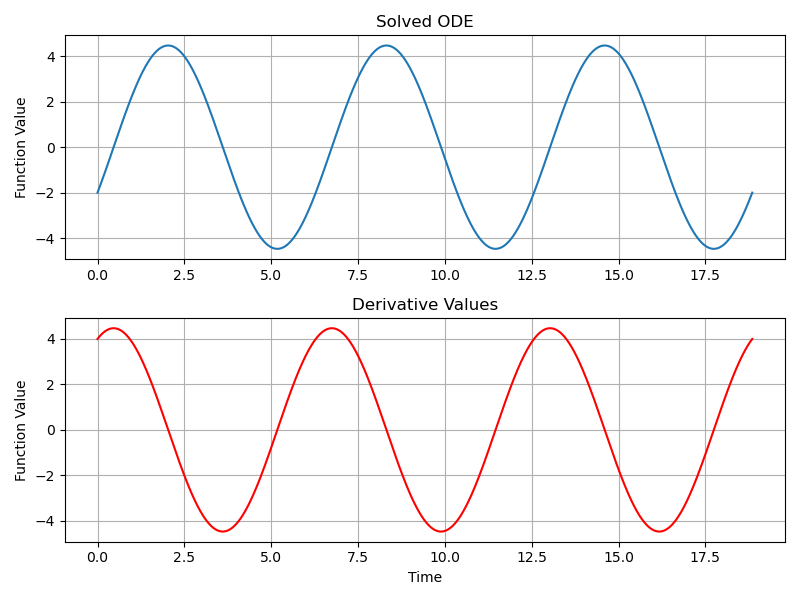
\includegraphics[width = \linewidth]{icml files/exp1.png}

\subsubsection{Spiral Approximation}
We also solved one of the problems specified in the paper - approximating spirals using neural ODEs. We created different types of spirals and tabulated the loss of our prediction w.r.t. the ground truth. We then trained our neural ODE network to fit the generated spiral and over many iterations, we can see the predicted spiral converging to the actual generated spiral. We ran several experiments with hyper parameters to test the robustness of our model. Here is one example of a spiral created by us for predictive modeling purposes:

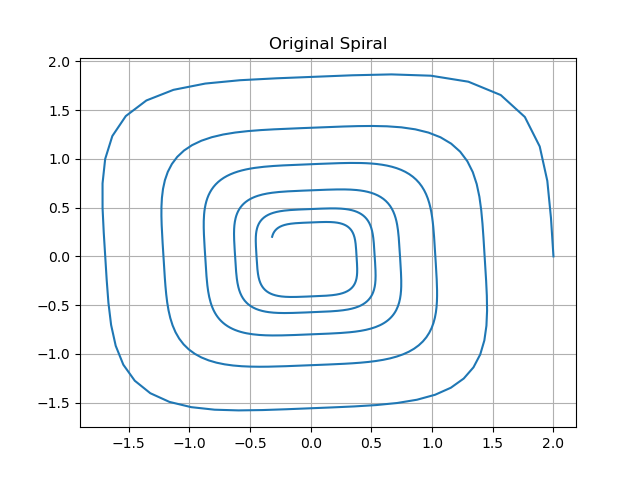
\includegraphics[width = \linewidth]{icml files/orig_spiral.png}

Here is the predicted spiral generated by our model:
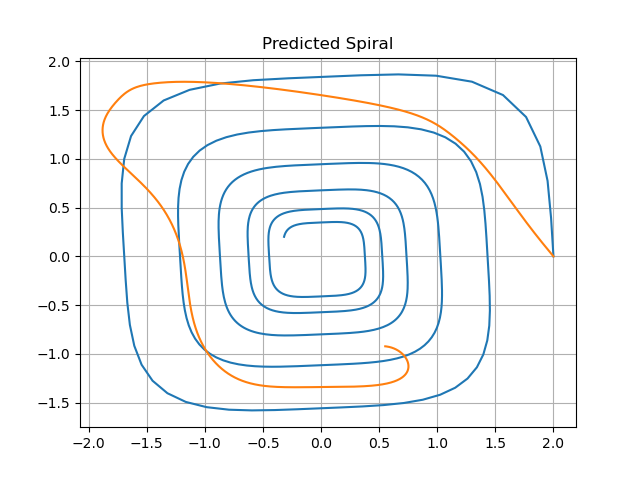
\includegraphics[width = \linewidth]{icml files/pred_spiral.png}

Here is another spiral and the progression of model fitting (Note that the predicted curve starts out random but is able to converge to the actual shape in a reasonable amount of iterations): 
\\
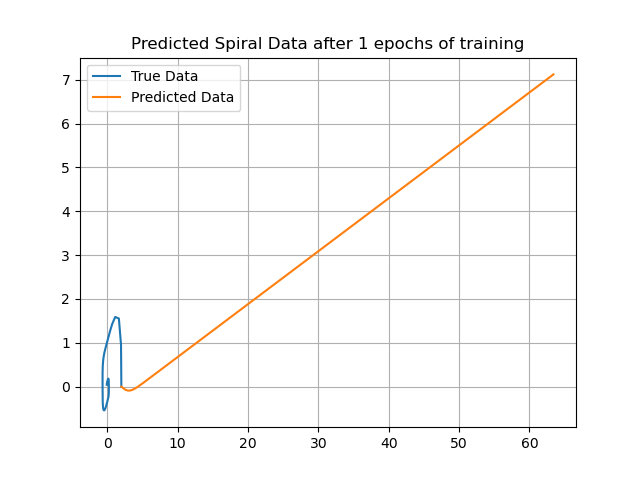
\includegraphics[width = 0.48\linewidth, valign=m]{icml files/pred_spiral_1.png} 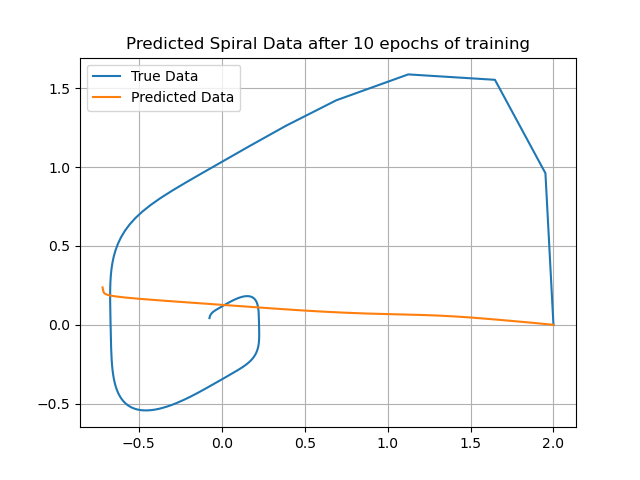
\includegraphics[width = 0.48\linewidth, valign=m]{icml files/pred_spiral_10.png}

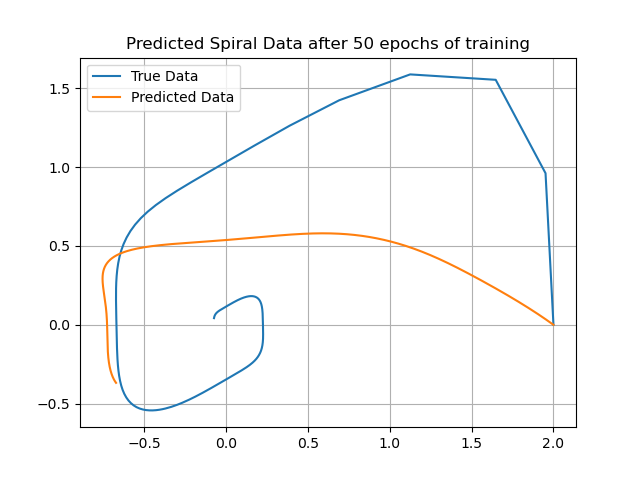
\includegraphics[width = 0.48\linewidth, valign=m]{icml files/pred_spiral_50.png} 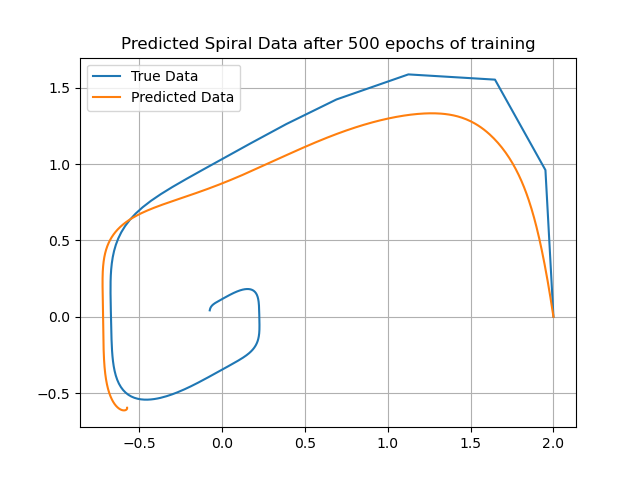
\includegraphics[width = 0.48\linewidth, valign=m]{icml files/pred_spiral_500.png}



\section{Contribution Statement}
\begin{itemize} 
    \item Shivam Duhan - Wrote all of 1.2, 3.1, added last part of 1.3, wrote parts of 2.1, 2.3, 2.4.
    \item Adam Piaseczny - Wrote first part of 1.1. Parts of 2.1, 2.2. Modified writing in 2.4. Wrote most of the code for the toy problem solution.
    \item Faaiz Memom - Wrote last part of 1.1, input to 2.1, parts of 2.4. Wrote some of the code for the toy problem solution.
    \item So Won Kim - Wrote first two parts of 1.3, wrote parts of 2.3, parts of 2.4. Helped with figure generation and placement for 3.1.
\end{itemize}
    

\end{document}



